\documentclass[11pt,class=report,crop=false]{standalone}
\usepackage[screen]{../python}


\begin{document}


%====================================================================
\chapitre{Fractale de Lyapunov}
%====================================================================

\index{fractale!fractale de Lyapunov}

\objectifs{Dans une contrée lointaine, des loups se nourrissent des ressources de la région. Chaque année des loups naissent, d'autres meurent, parfois la population des loups reste stable d'une année sur l'autre. Mais d'autres fois la population augmente, ce qui fait qu'il n'y a plus assez de nourriture pour tous, ainsi beaucoup de loups meurent et l'année suivante il y a peu de loups. Mais alors les quelques loups qui restent disposent de beaucoup de nourriture et se reproduisent rapidement, la population augmente et bientôt il y a trop de loups\ldots}

\bigskip

\begin{center}
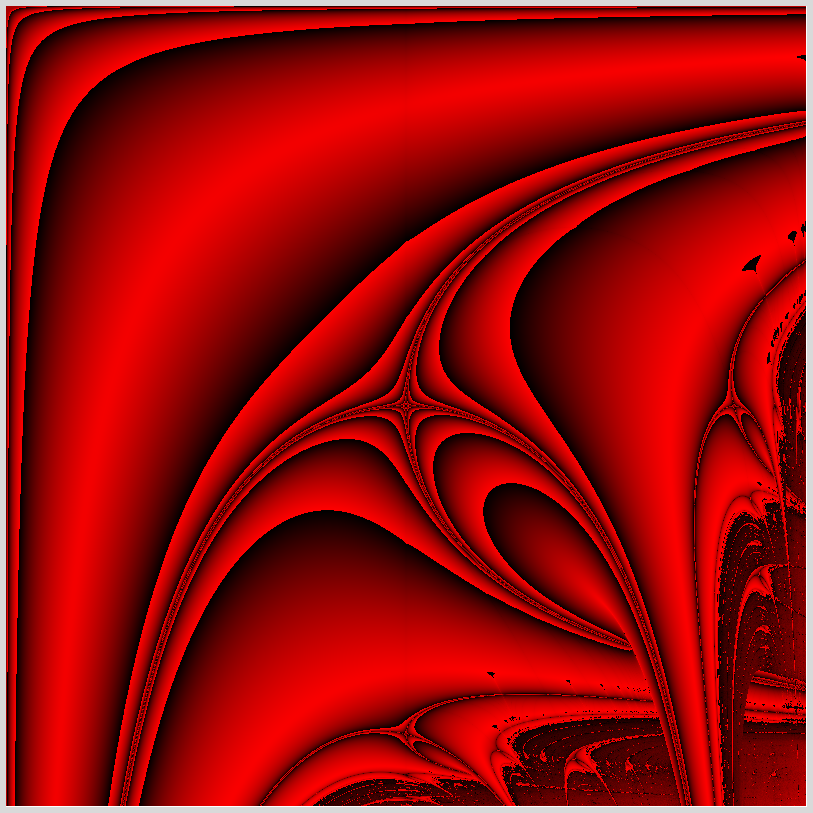
\includegraphics[scale=\myscale,scale=0.25]{ecran-lyapunov-AB}
\end{center}

\bigskip

\objectifs{Nous allons étudier des suites dont le comportement peut être chaotique. La fonction logarithme nous aidera à déterminer le caractère stable ou instable de la suite. Avec beaucoup de calculs et de patience nous tracerons des fractales très différentes de l'ensemble de Mandelbrot : les fractales de Lyapunov.}



%\begin{center}
%\couleurnb{
%
\includegraphics[scale=0.3]{ecran-mandelbrot-1}
%}
%{
%
\includegraphics[scale=0.3]{ecran-mandelbrot-1-nb}
%}
%\end{center}



%%%%%%%%%%%%%%%%%%%%%%%%%%%%%%%%%%%%%%%%%%%%%%%%%%%%%%%%%%%%%%%%
%%%%%%%%%%%%%%%%%%%%%%%%%%%%%%%%%%%%%%%%%%%%%%%%%%%%%%%%%%%%%%%%

\begin{cours}[La suite logistique]

\index{suite!logistique}
	
La suite logistique est une suite mystérieuse définie par récurrence.
On fixe d'abord un réel $r$ avec $0 \le r \le 4$. Il y a une suite pour chaque paramètre $r$.
La suite \defi{suite logistique de paramètre $r$} est la suite $(u_n)_{n\in\Nn}$ définie par récurrence :
$$u_0 = \frac12 
\qquad \text{ et } \qquad
u_{n+1} = r \cdot u_n \cdot (1-u_n) \quad \text{ pour } n\ge0.$$

\emph{Exemples.}
\begin{itemize}
  \item Fixons $r=\frac12$.
  Alors les premiers termes de la suite sont :
  $$u_0 = \frac12 \qquad 
  u_1 = \frac12 \frac12 \left(1-\frac12\right) = \frac18 \qquad
  u_2 = \frac12 \frac18 \left(1-\frac18\right) = \frac 7{128}$$
  $$
  u_3 = \frac12 \frac 7{128} \left(1-\frac7{128}\right) = 0.0258\ldots \qquad 
  u_4 = 0.0125\ldots$$ 
  
  La suite semble tendre vers $0$.
  
  \item Fixons $r=\frac32$.
  Alors les premiers termes de la suite sont :
  $$u_0 = \frac12 \qquad 
  u_1 = \frac32 \frac12 \left(1-\frac12\right) = \frac38 = 0.375 \qquad
  u_2 = \frac32 \frac38 \left(1-\frac38\right) = 0.351\ldots$$
  $$
  u_3 = 0.341\ldots \qquad 
  u_4 = 0.337\ldots$$ 
  
  La suite semble tendre vers $\frac13$.
  
  \item Fixons $r=3.2$. Voici les premiers termes de la suite :
$$	\begin{array}{lcl}
u_0 = 0.5 &\qquad& u_1 = 0.8 \\
u_2 = 0.512 &\qquad& u_3 = 0.79953\ldots \\
u_4 = 0.51288\ldots &\qquad& u_5 = 0.79946\ldots \\
u_6 = 0.51301\ldots &\qquad& u_7 = 0.799457\ldots \\
u_8 = 0.51304\ldots &\qquad& u_9 = 0.799455\ldots \\		
	\end{array}$$  
La suite $(u_n)$ n'a apparemment pas de limite, mais cependant les termes de rang pair $u_{2n}$ tendent vers une valeur $0.51304\ldots$, alors que les termes de rang impair $u_{2n+1}$ tendent vers une valeur $0.79945\ldots$
\end{itemize}

\bigskip


\emph{Les loups.}
La valeur de $u_n$ représente la population de loups à l'année $n$. Si $u_n=0$ il n'y a plus de loups, si $u_n=1$ il y a le maximum de loups. Le paramètre $r$ représente la vitesse de reproduction des loups (il ne change pas d'une année sur l'autre). La relation $u_{n+1} = r \cdot u_n \cdot (1-u_n)$ implique en particulier que si $u_n$ est proche de $0$ ou proche de $1$ alors $u_{n+1}$ est proche de $0$.

Reprenons les exemples un par un :
\begin{itemize}
  \item $r=0.5$. Les loups ne se reproduisent pas assez, la population finit par disparaître.
  \item $r=\frac32$. La population de loups finit par se stabiliser.
  \item $r=3.2$. La population ne se stabilise pas mais oscille entre deux valeurs d'une année sur l'autre.  
\end{itemize}

\end{cours}



\begin{cours}[Points d'accumulation]
Dans les exemples précédents on s'aperçoit que pour $r=0.5$ ou bien $r=1.5$ la suite $(u_n)$ possède une limite. Par contre, pour $r=3.2$ la suite $(u_n)_{n\in\Nn}$ n'a pas de limite. 
On pourrait presque dire que dans ce cas la suite $(u_n)$ possède deux limites, mais on s'interdit cet usage, car si une limite existe elle doit être unique.

Dans le cas $r=3.2$ on dit que la suite $(u_n)$ possède deux \defi{points d'accumulation} (ce sont les valeurs \og{}limites\fg{} $0.51304\ldots$ et $0.79945\ldots$).

Voici comment on va obtenir une approximation des points d'accumulation.
On calcule les premiers termes de la suite $(u_n)$ mais on ne retient que les termes $u_{100}$,
$u_{101}$, \ldots, $u_{199}$. Ces valeurs donnent une bonne approximation des points d'accumulation possibles.


Dans le cas $r=0.5$, la suite $(u_n)$ tend très vite vers $0$, ainsi tous les termes de $u_{100}$,
à $u_{199}$ sont quasiment nuls. Ils approchent donc bien la limite qui est $\ell=0$ (c'est le seul point d'accumulation).

\myfigure{0.6}{
\tikzinput{fig-lyapunov-1a}
}

Dans le cas $r=1.5$, la suite $(u_n)$ tend très vite vers $\frac13$, ainsi tous les termes de $u_{100}$, à $u_{199}$ approchent bien la limite qui est $\ell=\frac13$.

\myfigure{0.6}{
\tikzinput{fig-lyapunov-1b}
}    

Dans le cas $r=3.2$, les termes $u_{100}$ à $u_{199}$ alternent entre des valeurs
proches de chacun des deux points d'accumulation $\ell_1=0.51304\ldots$ et $\ell_2=0.79945\ldots$

\myfigure{0.6}{
\tikzinput{fig-lyapunov-1c}
}

Dans le cas $r=3.5$, la suite possède quatre points d'accumulation 
$\ell_1=0.50088\ldots$, $\ell_2=0.87499\ldots$,
$\ell_3=0.38281\ldots$ et $\ell_4=0.82694\ldots$

Conclusion : pour trouver une valeur approchée d'une limite ou des points d'accumulation, on se contente des valeurs de la suite de $u_{100}$ à $u_{199}$.

\end{cours}

%%%%%%%%%%%%%%%%%%%%%%%%%%%%%%%%%%%%%%%%%%%%%%%%%%%%%%%%%%%%%%%%
% Activité 1
%%%%%%%%%%%%%%%%%%%%%%%%%%%%%%%%%%%%%%%%%%%%%%%%%%%%%%%%%%%%%%%%

\begin{activite}[]

\objectifs{Objectifs : tracer les points d'accumulation de la suite logistique.}

\begin{center}
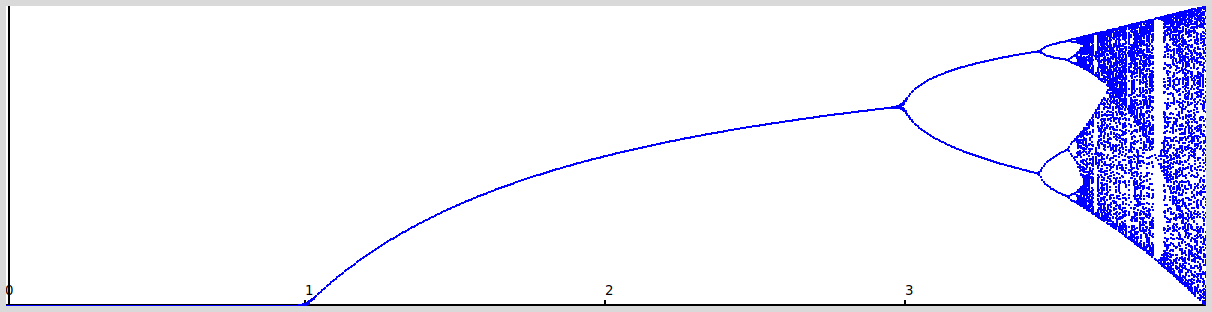
\includegraphics[scale=\myscale,scale=0.3]{ecran-lyapunov-1}
\end{center}

On rappelle que la suite logistique est définie pour un paramètre $0\le r \le 4$ par :
$$u_0 = \frac12 
\qquad \text{ et } \qquad
u_{n+1} = r \cdot u_n \cdot (1-u_n) \quad \text{ pour } n\ge0.$$

\begin{enumerate}
  \item Programme une fonction \ci{liste_suite(r,Nmin,Nmax)} qui renvoie la liste des termes de la suite logistique $u_n$ pour $n$ variant de $N_{\min}$ à $N_{{\max}}-1$.
  
  Par exemple  \ci{liste_suite(1.5,0,5)} renvoie les $5$ premiers termes de la suite définie par le paramètre $r=1.5$ : $[0.5, 0.375, 0.35156\ldots, 0.34194\ldots, 0.33753\ldots]$.
  
  
  \item  Programme une fonction \ci{bifurcation(Nmin,Nmax,epsilon)} qui renvoie la liste des points $(r,u_n)$ où :
  \begin{itemize}
    \item $r$ est un paramètre réel qui varie de $0$ à $4$, par saut de longueur $\epsilon$,
    \item $n$ est un entier qui varie de $N_{\min}$ à $N_{{\max}}-1$,
    \item $u_n$ est le terme de la suite logistique de paramètre $r$.
  \end{itemize}
  
  Par exemple avec $N_{\min} = 0$ à $N_{\max} = 5$ et $\epsilon = 1$, la fonction \ci{bifurcation()} renvoie la liste des points :

\begin{center}  
  \texttt{[(0, 0.5), (0, 0.0), (0, 0.0), (0, 0.0), (0, 0.0), \\
  (1, 0.5), (1, 0.25), (1, 0.1875), (1, 0.15234375), (1, 0.1291351318359375), \\
  (2, 0.5), (2, 0.5), (2, 0.5), (2, 0.5), (2, 0.5), \\
  (3, 0.5), (3, 0.75), (3, 0.5625), (3, 0.73828125), (3, 0.5796661376953125), \\
  (4, 0.5), (4, 1.0), (4, 0.0), (4, 0.0), (4, 0.0)]
  }
\end{center}
correspondant aux premiers termes des suites pour $r=0,1,2,3,4$.

  \item Affiche les points d'accumulation approchés $(r,u_n)$ 
  pour obtenir le diagramme de bifurcation.
  On prendra  $N_{\min} = 100$ à $N_{\max} = 200$ et $\epsilon = 0.01$. 
  Pour obtenir plus de points, on diminuera la valeur de $\epsilon$.
  
  
\end{enumerate} 

\begin{center}
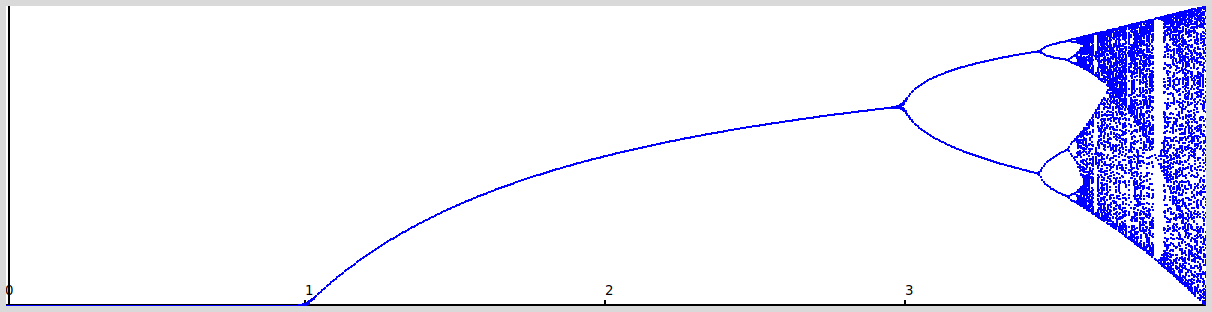
\includegraphics[scale=\myscale,scale=0.3]{ecran-lyapunov-1}
\end{center}

L'axe horizontal correspond aux valeurs de $r \in [0,4]$.
L'axe vertical correspond aux valeurs de $u_n \in [0,1]$.
Chaque point $(r,u_n)$ approche un point d'accumulation de la suite $(u_n)$ de paramètre $r$.

\bigskip


\begin{center}
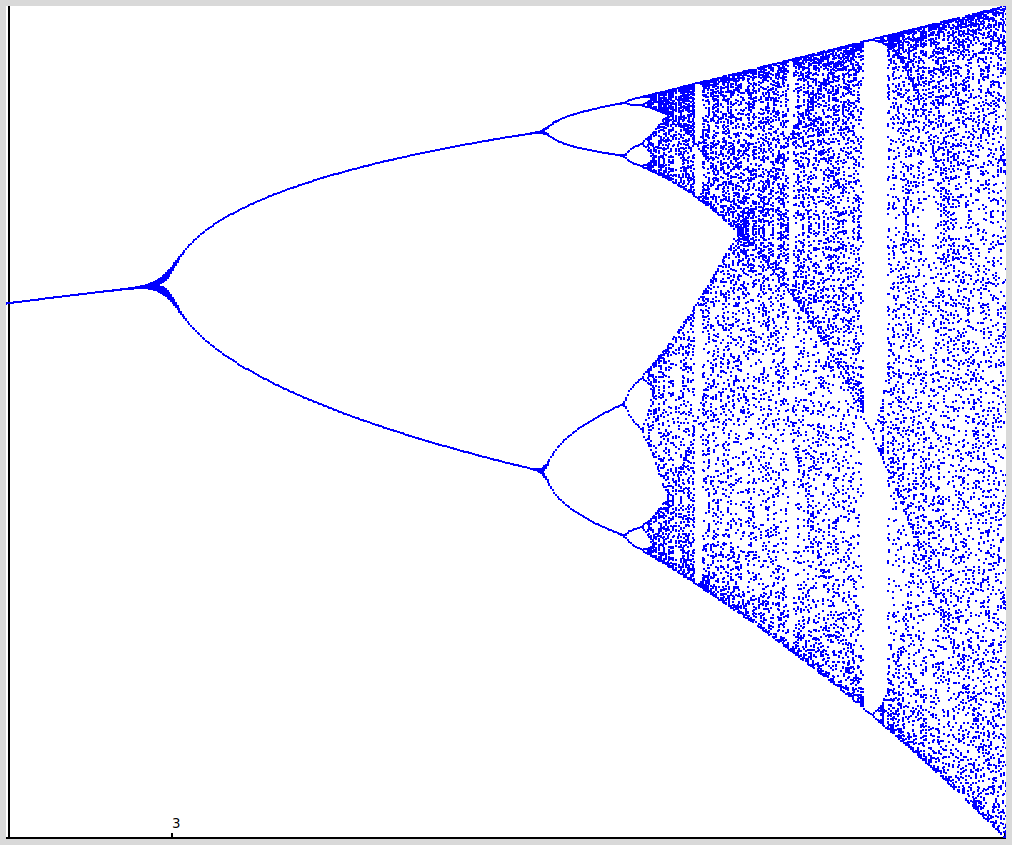
\includegraphics[scale=\myscale,scale=0.3]{ecran-lyapunov-2}

\emph{Zone où $r \ge 2.8$.}

\end{center}

\bigskip

\begin{center}
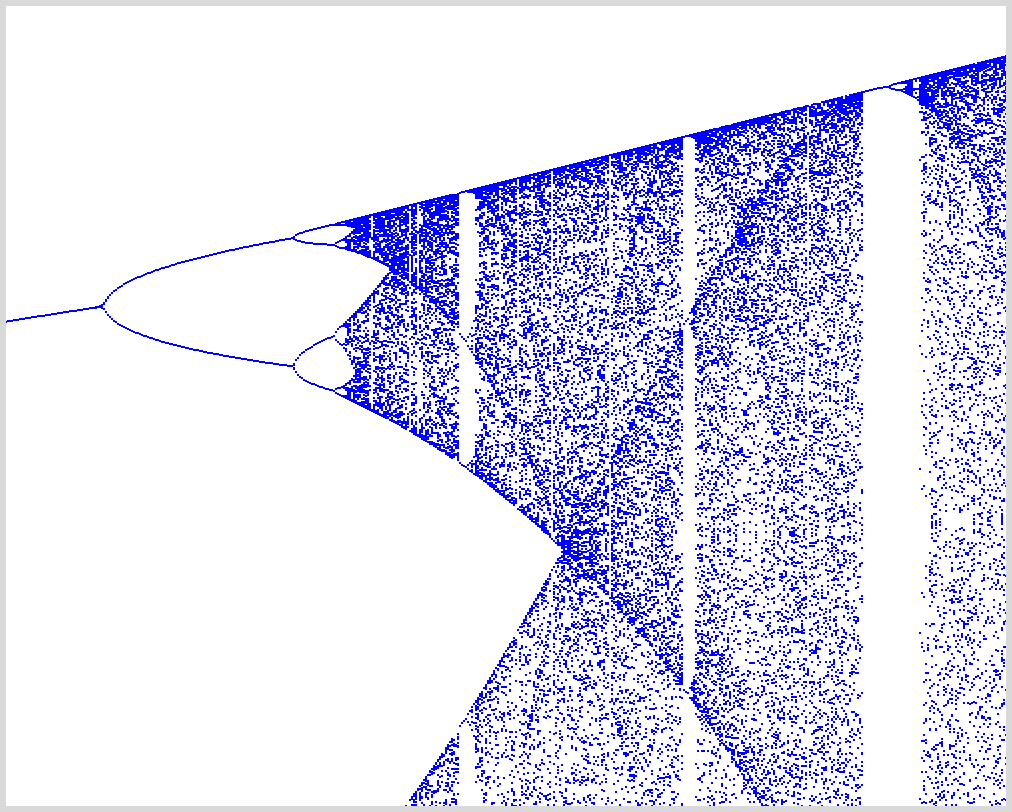
\includegraphics[scale=\myscale,scale=0.3]{ecran-lyapunov-3}

\emph{Zoom sur la zone où $r \in [3.3,3.9]$ et $u_n \in [0.6,1]$.}
\end{center}

\end{activite}


%%%%%%%%%%%%%%%%%%%%%%%%%%%%%%%%%%%%%%%%%%%%%%%%%%%%%%%%%%%%%%%%
%%%%%%%%%%%%%%%%%%%%%%%%%%%%%%%%%%%%%%%%%%%%%%%%%%%%%%%%%%%%%%%%

\begin{cours}[L'exposant de Lyapunov]

\objectifs{L'exposant de Lyapunov mesure la stabilité de nos suites logistiques. Plus l'exposant est négatif plus la suite est stable, plus l'exposant est positif plus la suite est chaotique.}


\textbf{Définition générale.}

Considérons une suite $(u_n)_{n\in\Nn}$ définie par un terme initial et une formule de récurrence
$$u_0\in \Rr \qquad \text{ et } \qquad u_{n+1} = f(u_n)$$
où $f : \Rr \to \Rr$ est une fonction.

L'\defi{exposant de Lyapunov} associé à cette suite est :
$$L = \lim_{N\to+\infty} \frac1N \sum_{n=0}^{N-1} \ln\left( \big| f'(u_n) \big| \right)$$
\index{logarithme}

C'est une moyenne de logarithmes. On va expliquer plus bas comment calculer cette formule compliquée dans notre cas.

\bigskip

\textbf{L'exposant de Lyapunov approché pour la suite logistique.}

Dans notre cas la suite logistique est définie à l'aide de la fonction $f(x) = rx(1-x)$, pour laquelle $f'(x) = r - 2rx$, de sorte que pour $N$ assez grand :
$$L_r \ \simeq \ \frac 1N  \sum_{n=0}^{N-1}  \ln\left(\big| r-2ru_n  \big| \right)$$
c'est-à-dire
$$L_r \simeq \frac 1N \left( 
\ln\left(\big| r-2ru_0  \big| \right) + 
\ln\left(\big| r-2ru_1  \big| \right) + \cdots +
\ln\left(\big| r-2ru_n  \big| \right) + \cdots +
\ln\left(\big| r-2ru_{N-1}  \big| \right)
\right)$$ 

Attention ! Il faut supposer $r>0$. Il faut aussi exclure de cette somme les termes $u_n=\frac12$ (car le logarithme n'est pas défini en $0$).

%\bigskip
%
%\textbf{Calcul pratique.}
%Pour approcher efficacement la limite dans la pratique nous ne retiendrons que les termes entre $N_{\min}$ à $N_{\max}$
%$$L_r \simeq \frac 1N  \sum_{n=N_{\min}}^{N_{\max}-1}  \ln\left(\big| r-2ru_n  \big| \right)$$ 
%où $N = N_{\max} - N_{\min}$ est le nombre de termes de la somme.



\end{cours}


%%%%%%%%%%%%%%%%%%%%%%%%%%%%%%%%%%%%%%%%%%%%%%%%%%%%%%%%%%%%%%%%
% Activité 2
%%%%%%%%%%%%%%%%%%%%%%%%%%%%%%%%%%%%%%%%%%%%%%%%%%%%%%%%%%%%%%%%

\begin{activite}[Exposant de Lyapunov]

\objectifs{Objectifs : calculer l'exposant de Lyapunov et le visualiser.}

\begin{center}
\couleurnb{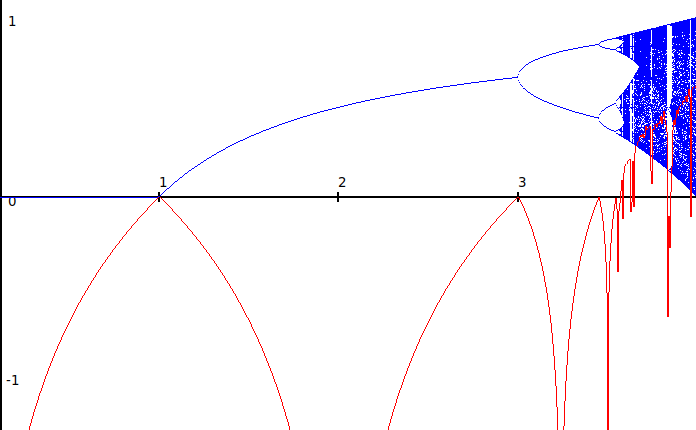
\includegraphics[scale=\myscale,scale=0.5]{ecran-lyapunov-8-coul}}{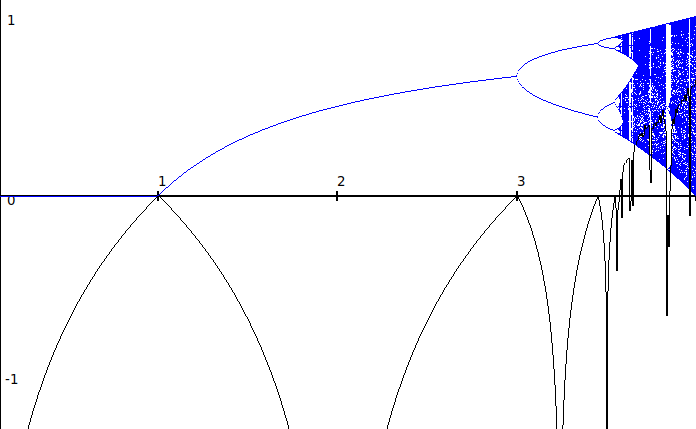
\includegraphics[scale=\myscale,scale=0.5]{ecran-lyapunov-8-nb}}

\end{center}

\begin{enumerate}
  \item  Programme une fonction \ci{exposant_lyapunov(liste_u,r)}
  qui renvoie une valeur approchée de l'exposant de Lyapunov selon la formule :
$$L_r \simeq \frac{1}{N} \sum_{u \in \text{liste}}  \ln\left(\big| r-2 r u  \big| \right)$$
où $N$ est le nombre d'éléments de la liste.

 \emph{Indication.} N'oublie pas d'exclure de la somme les cas où $u=\frac12$ .
 
  \item Programme une fonction \ci{bifurcation_lyapunov()} qui 
  affiche le graphe de la fonction $r \mapsto L_r$.
  
  \emph{Indications.}
\begin{itemize}
  \item Voir le tracé \couleurnb{(en rouge) }{}sur la figure ci-dessus.

  \item Autrement dit, il faut afficher les points $(r,L_r)$ pour $r$ variant de $0$ à $4$ par exemple.
  
  \item Il vaut mieux ici relier les points correspondant $(r,L_r)$ à $(r+\epsilon,L_{r+\epsilon})$, avec un petit pas $\epsilon$, pour obtenir un plus joli tracé.
  
  \item C'est encore mieux de tracer ce graphe sur le même graphique que le diagramme de bifurcation.
  
  \item Pour approcher efficacement la limite dans la formule de l'exposant de Lyapunov il est conseillé de ne retenir que les termes de rang $N_{\min}$ à $N_{\max}-1$, avec par exemple 
comme auparavant  $N_{\min}=100$ et $N_{\max}=200$.
\end{itemize}  
  
  
\end{enumerate} 


\bigskip{Exemples.}

\begin{itemize}
  \item $r=0.5$. Si on calcule l'exposant de Lyapunov en se limitant aux premiers termes $[u_0,u_1,\ldots,u_{9}]$ alors on trouve $L_{0.5} \simeq -0.67$.
  Pour une meilleure approximation, on calcule la somme avec les termes $u_{100}$ à $u_{199}$ (donc avec $N_{\min}=100$ à $N_{\max}=200$), on trouve $L_{0.5} \simeq -0.69$.
  Un exposant négatif correspond à une situation stable : ici la suite tend vers $0$. 
  
  \item $r=3$. On trouve $L_3 = 0$. L'exposant est nul, la situation n'est pas très stable (pour $r<3$ la suite a une limite, pour $r$ juste plus grand que $3$ la suite possède deux points d'accumulation).
  
    \item $r=3.2$. On trouve $L_{3.2} \simeq -0.91$. C'est une situation stable, même si la suite ne converge pas ses valeurs oscillent régulièrement entre deux valeurs limites.
  
  \item $r=3.7$. On trouve $L_{3.7} \simeq 0.32$. L'exposant est positif, nous sommes dans la zone chaotique.
  
\end{itemize}

\end{activite}



%%%%%%%%%%%%%%%%%%%%%%%%%%%%%%%%%%%%%%%%%%%%%%%%%%%%%%%%%%%%%%%%
%%%%%%%%%%%%%%%%%%%%%%%%%%%%%%%%%%%%%%%%%%%%%%%%%%%%%%%%%%%%%%%%

\begin{cours}[Suite logistique suivant un motif]

\textbf{Motif.} 
\begin{itemize}
  \item Un \defi{motif} est une suite de lettres \mot{A} ou \mot{B}, par exemple \mot{AB} ou \mot{AABA}.
  \item En répétant un motif, on obtient un mot de longueur infinie, par exemple avec
  \mot{AB} on obtient \mot{AB\,AB\,AB\,AB\,AB\,\ldots} et avec \mot{AABA} on obtient \mot{AABA\,AABA\,AABA\,\ldots}
  \item La $n$-ème lettre tirée d'un motif est la $n$-ème lettre du mot infini issu du motif (en commençant avec $n=0$). Par exemple pour le motif \mot{AB}, pour $n$ pair la lettre est \mot{A} et $n$ impair la lettre est \mot{B}. Pour le motif \mot{AABA} et $n=6$ la lettre est \mot{B}.
\end{itemize}

\bigskip

\textbf{Suite logistique d'après un motif.}
On va définir une suite logistique à deux paramètres.
\begin{itemize}
  \item On fixe deux valeurs réelles $r_1$ et $r_2$ dans l'intervalle $[0,4]$.
  \item On fixe un motif.
  \item On initialise une suite à $u_0 = \frac12$.
  \item La suite logistique de paramètres $(r_1,r_2)$ est définie par récurrence :
  \begin{itemize}
    \item si la $n$-ème lettre issue du motif est \mot{A} alors $u_{n+1} = r_1u_n(1-u_n)$,
    \item si la $n$-ème lettre issue du motif est \mot{B} alors $u_{n+1} = r_2u_n(1-u_n)$.
  \end{itemize}
  
\bigskip

\textbf{Exemple.} 
Calculons la suite logistique avec le motif \mot{AB} et les paramètres $(\frac12,\frac72) = (0.5,3.5)$. 
Le motif donne le mot \mot{AB\,AB\,AB\,AB\,AB\ldots} on va donc alterner le paramètre $r_1$ et le paramètre $r_2$.
\begin{itemize}
  \item $u_0 = \frac 12$ (terme initial),
  \item $n=0$, la lettre de rang $0$ est \mot{A}, donc $u_1 = r_1 u_0 (1-u_0) = \frac18 = 0.125$.
  \item $n=1$, la lettre de rang $1$ est \mot{B}, donc 
  $u_2 = r_2 u_1 (1-u_1) = 0.382\ldots$
  \item $n=2$, la lettre de rang $2$ est \mot{A}, donc $u_3 = r_1 u_2 (1-u_2) = 0.118\ldots$
  \item $u_4 = r_2 u_3 (1-u_3) = 0.364\ldots$
  \item $u_5 = 0.115\ldots$
\end{itemize}

\end{itemize}



\end{cours}

%%%%%%%%%%%%%%%%%%%%%%%%%%%%%%%%%%%%%%%%%%%%%%%%%%%%%%%%%%%%%%%%
%%%%%%%%%%%%%%%%%%%%%%%%%%%%%%%%%%%%%%%%%%%%%%%%%%%%%%%%%%%%%%%%

\begin{cours}[Fractale de Lyapunov.]

Voici comment est définie une fractale de Lyapunov :
\begin{itemize}
  \item Tout d'abord on fixe un motif.
  \item La fractale est dessinée dans la zone $[0,4] \times [0,4]$, correspondant 
  aux paramètres $(r_1,r_2)$.
  \item Pour chacun des paramètres $(r_1,r_2)$ : 
  \begin{itemize} 
    \item on calcule la suite logistique associée à ces paramètres et au motif,
    \item on calcule l'exposant de Lyapunov de cette suite,
    \item on colorie le pixel $(r_1,r_2)$ en fonction de la valeur de l'exposant.
  \end{itemize} 
\end{itemize}
  
Si on change de motif on obtient une fractale un peu différente !



\end{cours}


%%%%%%%%%%%%%%%%%%%%%%%%%%%%%%%%%%%%%%%%%%%%%%%%%%%%%%%%%%%%%%%%
% Activité 3
%%%%%%%%%%%%%%%%%%%%%%%%%%%%%%%%%%%%%%%%%%%%%%%%%%%%%%%%%%%%%%%%

\begin{activite}[Fractale de Lyapunov]

\objectifs{Tracer les fractales de Lyapunov. Il est bon d'avoir déjà tracé la fractale de Mandelbrot, le principe étant similaire, mais ici les calculs sont beaucoup plus lents.}

\begin{center}
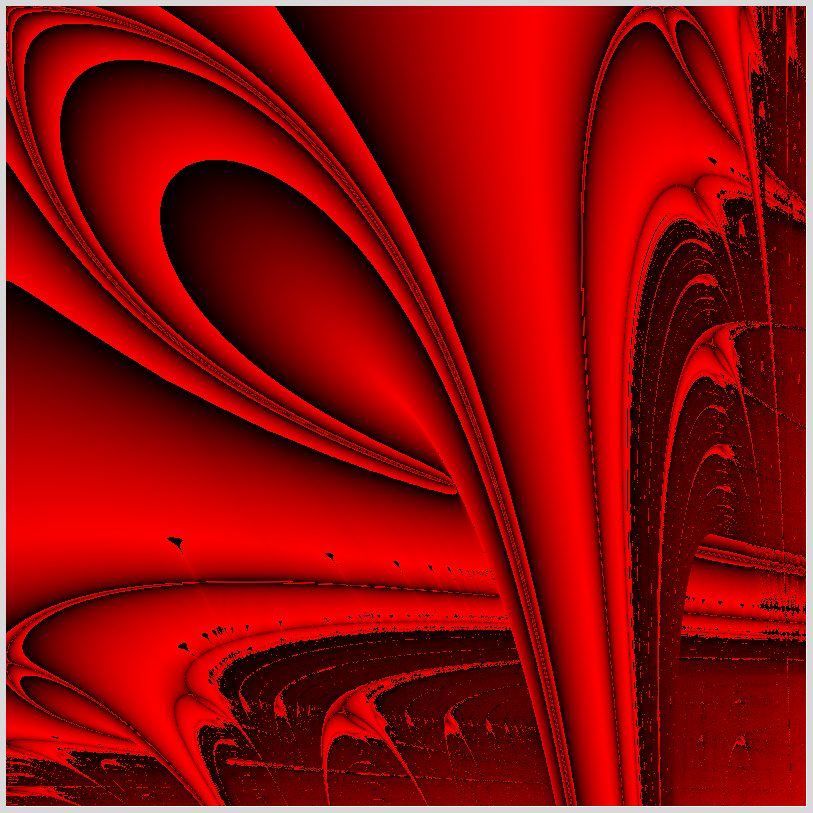
\includegraphics[scale=\myscale,scale=0.25]{ecran-lyapunov-AB-2-4-2-4}
\end{center}

\begin{enumerate}

  \item Programme une fonction \ci{A_ou_B(motif,n)} qui pour une chaîne \ci{motif}, renvoie le caractère \ci{'A'} ou \ci{'B'} de rang $n$ du mot itéré.
  
  \emph{Exemple.} \ci{A_ou_B('AB',10))} renvoie \ci{'A'} alors que 
  \ci{A_ou_B('AAABBB',123)} renvoie \ci{'B'}.
  
  \item Modifie ta fonction précédente en une fonction  \ci{liste_suite_motif(r1,r2,motif, Nmin,Nmax)} qui renvoie
  la suite logistique construite d'après le motif donné et les paramètres $(r_1,r_2)$ sous la forme d'une liste de termes $u_n$ avec $N_{\min} \le n < N_{\max}$.
  
  
  \emph{Exemple.} 
  Avec $r_1 = 0.5$ et $r_2 = 3.5$ et le motif \mot{AB} alors la commande 
  \ci{liste_suite_motif(r1,r2,motif,0,10)} renvoie les dix premiers termes de la suite logistique :
  \begin{center}
  \texttt{[0.5, 0.125, -1.0937\ldots, -0.273\ldots, 2.392\ldots, \\
  0.598\ldots, -5.233\ldots, -1.308\ldots, 11.448\ldots, 2.862\ldots]
  }\end{center}

  \item Modifie ta fonction précédente en une fonction  
  \mycenterline{\ci{exposant_lyapunov_motif(r1,r2,motif,Nmin,Nmax)}}
   qui calcule l'exposant de Lyapunov de la liste des termes de la suite logistique avec $N_{\min} \le n < N_{\max}$.
  
  \emph{Indications.} Reprends une partie du code de la fonction 
  \ci{exposant_lyapunov()} que tu intègres dans le code de ta fonction \ci{liste_suite_motif()}.
  
   \emph{Exemple.} 
  Prenons $r_1 = 0.5$ et $r_2 = 3.5$ et le motif \mot{AB} alors, 
  avec les $10$ premiers termes de la suite ($N_{\min}=0$, $N_{\max}=10$), on trouve un exposant de Lyapunov de $-0.506\ldots$ 
  Pour obtenir la valeur à la limite qui donne l'exposant, on prend en compte plus de termes, après avoir oublié les premiers termes, par exemple en posant $N_{\min}=100$, $N_{\max}=200$. On obtient alors un bonne approximation de l'exposant de Lyapunov de la suite logistique $L_{r_1,r_2} = -0.940147\ldots$
  
 
  \item Programme une fonction \ci{fractale_lyapunov(motif)} qui dessine la fractale de Lyapunov associée au motif.
  
  Suis l'algorithme suivant :
  \begin{itemize}
    \item Fixer la taille de la fenêtre $N$ en pixel ($N=100$ pour commencer car les calculs sont très longs).
    \item La fenêtre réelle étant la zone $[0,4]\times [0,4]$, fixer un pas $h$ défini par $h = 4/N$.
  
  \item Initialiser $r_1$ à $0$.
  \item Pour $i$ allant de $0$ à $N$ :
  \begin{itemize}
    \item Initialiser $r_2$ à $0$.
    \item Pour $j$ allant de $0$ à $N$ :
    \begin{itemize}
      \item calculer l'exposant de Lyapunov de la suite logistique associée au motif donné et aux paramètres $(r_1,r_2)$,
      \item colorier le pixel $(i,j)$ en fonction de cet exposant,
      \item faire $r_2 \leftarrow r_2 + h$.
    \end{itemize} 
    \item Faire $r_1 \leftarrow r_1 + h$.
  \end{itemize} 
\end{itemize}  
    

\myfigure{0.7}{
\tikzinput{fig-lyapunov-2}
}
    
    
\end{enumerate} 


\emph{Couleurs.} Voici  une fonction qui renvoie une couleur en fonction d'une valeur $\ell$ de l'exposant de Lyapunov.

\begin{lstlisting}
def choix_couleur(l):
    i = round(150*l)
    R,V,B = i,0,0     # Nuances de rouge
    couleur = '#%02x%02x%02x' % (R%256, V%256, B%256)
    return couleur
\end{lstlisting}  
    
\emph{Zoom.} Pour afficher une fenêtre précise correspondant à une zone plus petite que la zone $[0,4] \times [0,4]$ vois l'activité \og{}Ensemble de Mandelbrot\fg{}.

\bigskip

De gauche à droite les fractales de Lyapunov pour les motifs
\mot{AB},
\mot{AAABB},
\mot{AAAAABABBB}.

\begin{center}
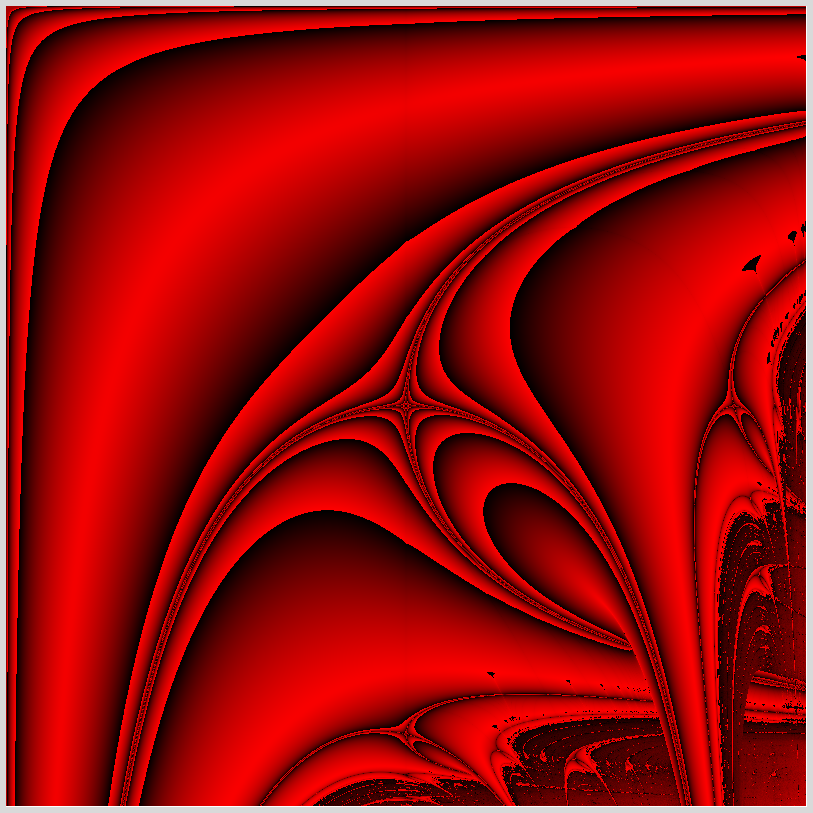
\includegraphics[scale=\myscale,scale=0.15]{ecran-lyapunov-AB}\quad
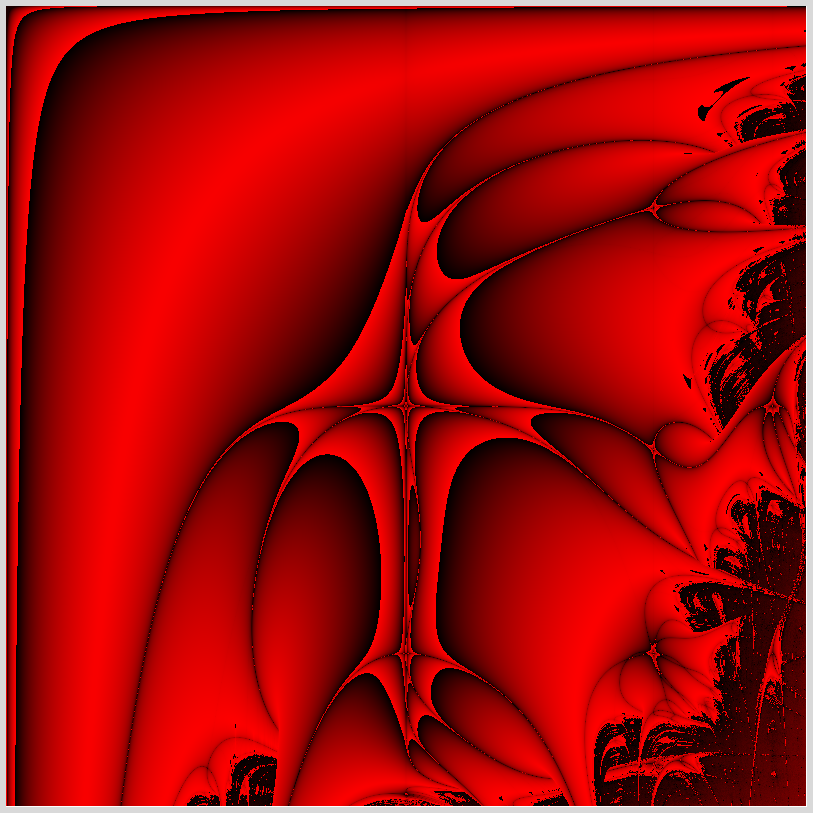
\includegraphics[scale=\myscale,scale=0.15]{ecran-lyapunov-AAABB}\quad
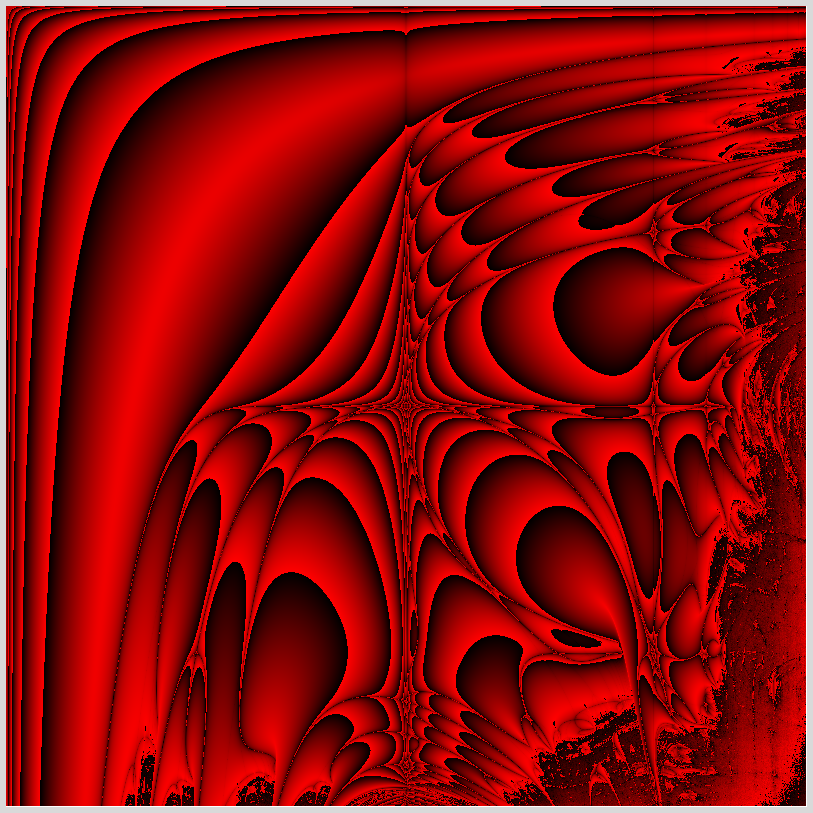
\includegraphics[scale=\myscale,scale=0.15]{ecran-lyapunov-AAAAABABBB}
\end{center}

Il est amusant d'explorer différents motifs, de changer la formule pour les couleurs et de faire des zooms sur les parties chaotiques.

Voici des zooms pour le motif \mot{AB}, à gauche sur la zone $[2,4]\times [2,4]$,
à droite sur la zone $[2,3]\times[3,4]$. 
\begin{center}
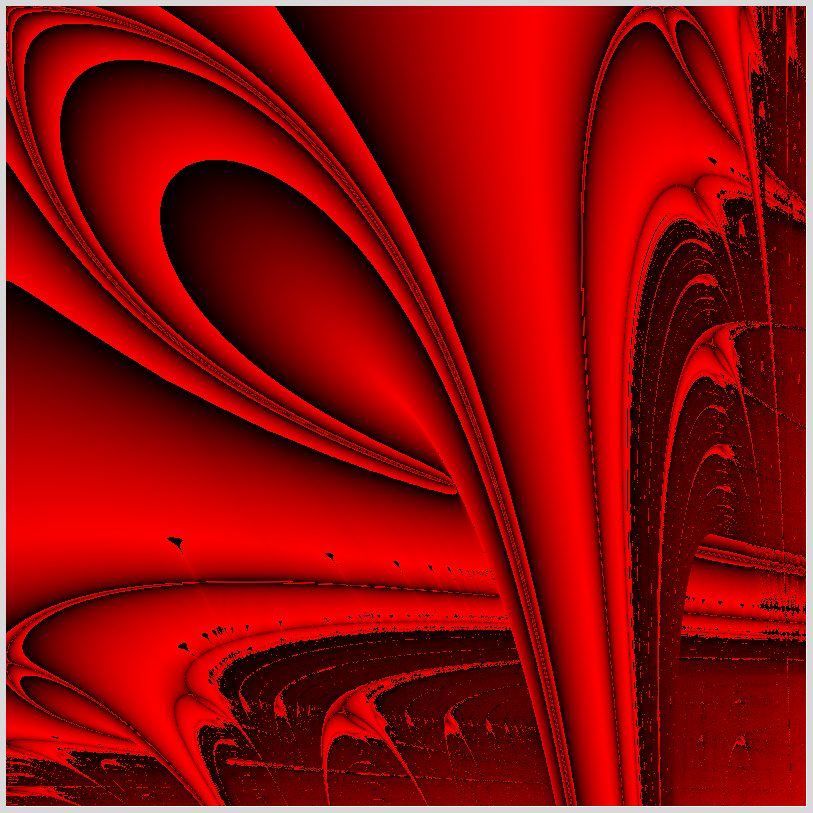
\includegraphics[scale=\myscale,scale=0.2]{ecran-lyapunov-AB-2-4-2-4}\quad
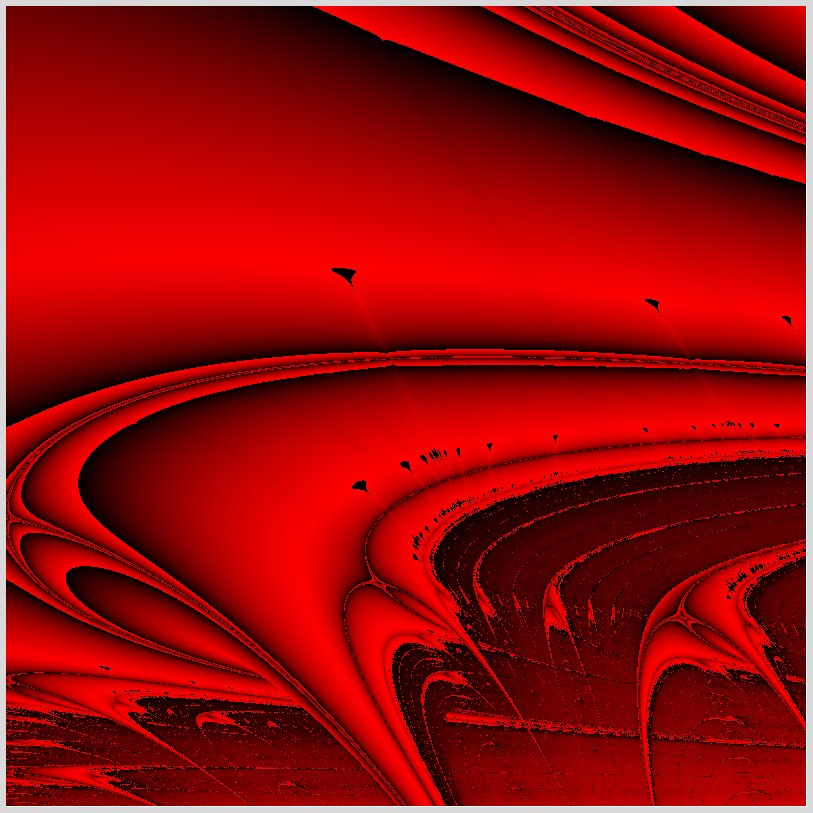
\includegraphics[scale=\myscale,scale=0.2]{ecran-lyapunov-AB-2-3-3-4}
\end{center}

\end{activite}


\end{document}
